\subsubsection{Design Approach}
We have chosen to use the Customer Insight\cite{1} techinique in our design approach. If we had the funds available, we could hire social scientists which could sketch profiles of the customer segment. As this is not the case, we have made use of the Empathy Map, which is also known as the ``really simple customer profiler''\cite{2}.

The first thing to do when using the empathy map, is to brainstorm all possible customer segments that one might want to serve with the business model. Then three promising candidates should be chosen, from which a single candidate is selected for the first profiling exercise. Then a customer from that customer segment is thought up, by giving the customer characteristics, such as a name, income, occupation, and so on. Afterwards a profile is build for the customer by asking and answering six questions.
These questions should be put on a whiteboard or flipchart, as seen in figure \ref{fig:empathy_map}(Hence, empathy map), and the answers could be written on stick-it notes and placed on the questions.

The six questions are\cite{2}:
\begin{itemize}
\item What does the customer see? Describe what the customer sees in their environment
\item What does the customer hear? Describe how the environment influences the customer
\item What does the customer really feel and think? Try to sketch out what goes on in their mind
\item What does the customer say and do? Imagine what the customer might say, or how the customer might behave in public
\item What is the customer's pain? E.g. what are their biggest frustrtations?
\item What does the customer gain? E.g. what does the customer truly want or need to achieve?
\end{itemize}

\begin{figure}[h]
    \begin{center}
        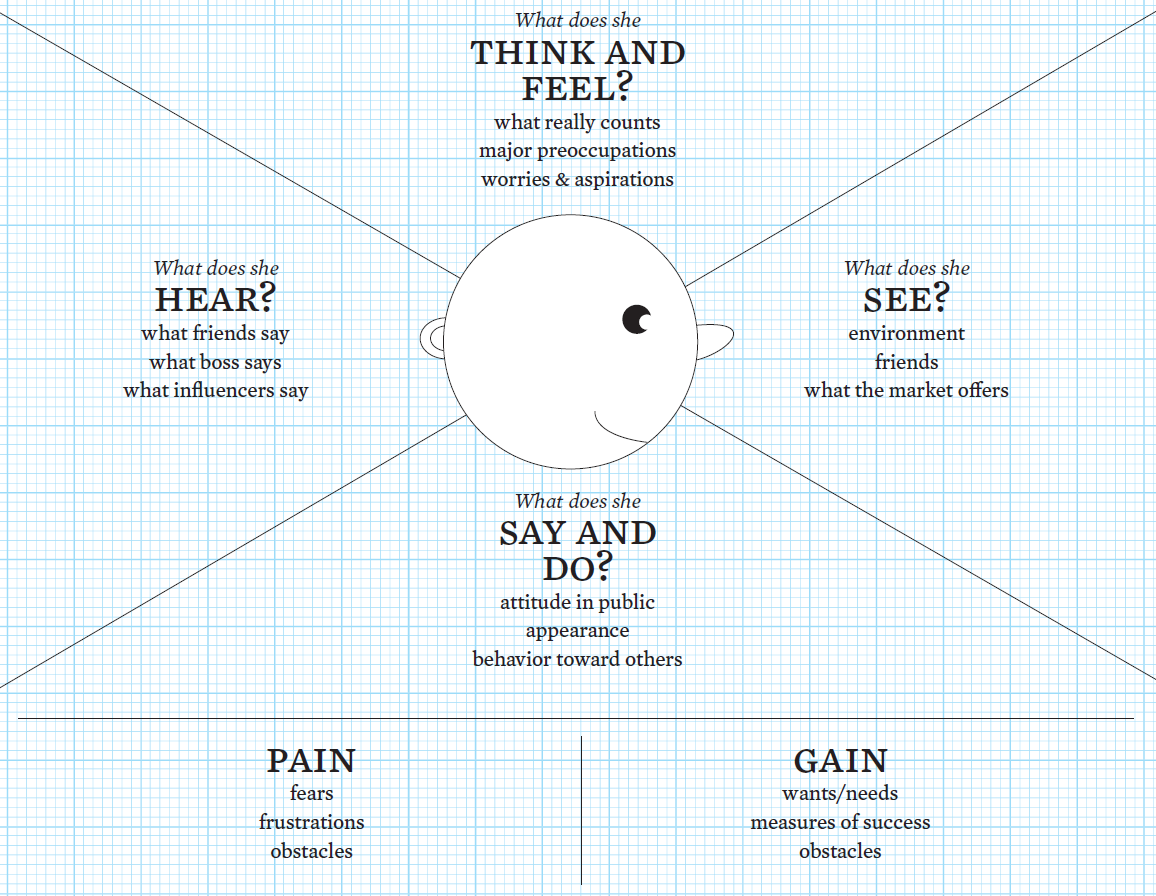
\includegraphics[scale=0.52]{./pics/empathy_map}
        \label{fig:empathy_map}
        \caption{Adapted empathy map from XPLANE\cite{3}}
    \end{center}
\end{figure}

The three candidate costumer segments we have come up with are:
\begin{enumerate}
\item Couples in the age range of 25-35, with children, that is ``forced'' to have cable because the children need their saturday morning cartoons.
\item Students in the age range of 18-24, not living at home, limited income e.g. support from the government. Illegally downloads movies and TV-shows, as they can't afford cable or to buy them.
\item People in the age range of 16-35, illegally downloads movies and TV-shows because of ease-of-access.
\end{enumerate}

We are basing our customer on candidate 2 from the list. He is called John, he has no income except for support from the government,

% 1: Business model generation, 127-133
% 2: Business model generation, 131
% 3: Business model generation, 130